\documentclass[11pt,a4paper]{report}

\usepackage[margin=0.6in]{geometry}
\usepackage{titlesec}% http://ctan.org/pkg/titlesec
\usepackage{lipsum}% http://ctan.org/pkg/lipsum
\usepackage{amsmath}
\usepackage{xcolor}
\usepackage{tikz}
\usepackage{bm}
\usepackage{times}
\usepackage{amsthm}
\usepackage[mathscr]{euscript}
\usepackage{hyperref}
\usepackage{mathtools}


% Tikz setup
\usetikzlibrary{arrows,shapes}

\title{Cryptography}
\author{Stephen O'Brien}

% Change amount of space after "Chapter" heading (<after-sep> param)
\titleformat{\chapter}{\Huge\bfseries}{\chaptername\ \thechapter}{0pt}{\vskip 20pt\raggedright}%
\titlespacing{\chapter}{0pt}{50pt}{10pt}% \titlespacing{<command>}{<left>}{<before-sep>}{<after-sep>}[<right>]

% Increase table row height globally
\renewcommand{\arraystretch}{2}

\newcommand\todo[1]{\noindent\textcolor{red}{TODO: #1}}

\newtheorem{definition}{Definition}
\newtheorem{theorem}{Theorem}[section]
\newtheorem{lemma}{Lemma}

\begin{document}
\maketitle
\chapter{Discrete Probability}
\begin{center}
		\emph{
			``If you think technology can solve your security problems, then you don't understand the problems and you don't understand the technology.'' - Bruce Shneier
		}
\end{center}



\section{Probability Distribution}
Let $U$ be a finite set (e.g. $U = \{0,1\}^n$), \textbf{probability distribution} $P$ over $U$ is a function $P : U \rightarrow [0,1]$ such that

\begin{gather}
	\sum\limits_{x \in  U} P(x) = 1
\end{gather}

\todo{Expand on what Probability Distribution is}

\subsection{Examples}
\subsubsection{Uniform Distribution}
\begin{gather}
	\forall . x \in U : P(x) = \frac{1}{|U|}
\end{gather}
\subsubsection{Point Distribution}
Point distribution at $x_0$:
\begin{gather}
	P(x_0) = 1, \forall.x \neq x_0 : P(x) = 0
\end{gather}

	
	
\section{Events}
For a set $A \subseteq U$:

\begin{gather}
	Pr[A] = \sum\limits_{x \in A} P(x) \in [0,1]		
\end{gather}
\begin{center}
	Note: $Pr[U] = 1$
\end{center}

\noindent
The set $A$ is called an \textbf{event}.

\subsection{Example}
Let $U = \{0,1\}^8$ ($|U| = 256$, all possible byte values).

\begin{gather*}
	A = \{ x \in U \;|\; lsb_2(x) = 11\} \subseteq U \\
	\textrm{for uniform distribution on } \{0,1\}^8 : Pr[A] = \frac{1}{4}
\end{gather*}


\section{The Union Bound}
For events $A_1$ and $A_2$:
\begin{gather*}
	Pr \big[A_1 \cup A_2 \big] \le Pr \big[A_1 \big] + Pr \big[A_2 \big]
\end{gather*}

\subsection{Example}
\begin{gather*}
	A_0 = \big\{ x \in \{0,1\}^n \;|\; lsb_2(x)=11 \big\} \quad ; \quad A_1 = \big\{ x \in \{0,1\}^n \;|\; msb_2(x)=11 \big\}	\\
		Pr \big[ lsb_2(x) = 11 \; \textrm{or} \; msb_2(x) = 11 \big] = Pr \big[A_0 \in A_1 \big] \leq \frac{1}{4} + \frac{1}{4} = \frac{1}{2}
\end{gather*}
\begin{center}
	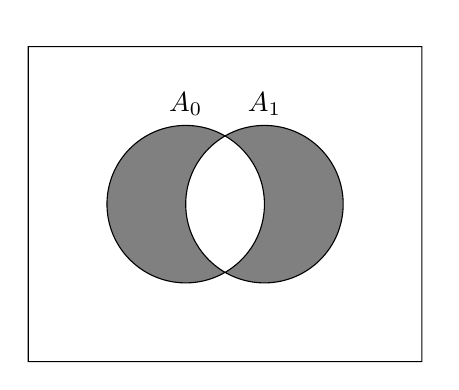
\begin{tikzpicture}[fill=gray]
	% left hand
	\scope
	\clip (-2,-2) rectangle (2,2)
	      (1,0) circle (1);
	\fill (0,0) circle (1);
	\endscope
	% right hand
	\scope
	\clip (-2,-2) rectangle (2,2)
	      (0,0) circle (1);
	\fill (1,0) circle (1);
	\endscope
	% outline
	\draw (0,0) circle (1) (0,1)  node [text=black,above] {$A_0$}
	      (1,0) circle (1) (1,1)  node [text=black,above] {$A_1$}
	      (-2,-2) rectangle (3,2) node [text=black,above] {};
	\end{tikzpicture}
\end{center}


\section{Random Variables}
A random variable $X$ is a function $X : U \rightarrow V$

\subsection{Example}
\begin{gather*}
X : \{ 0,1 \}^n \rightarrow \{ 0,1 \} \; ; \; X(y) = lsb(y) \in \{0,1\}
\end{gather*}

\noindent
For the uniform distribution on $U$:
\begin{gather*}
	Pr [X=0] = \frac{1}{2} \; , \; Pr [X=0] = \frac{1}{2}
\end{gather*}

\noindent
More generally, rand. var $X$ induces a distribution on $V$: 
\begin{gather*}
	Pr [X=v] := Pr \big[ X^{-1}(v) \big]
\end{gather*}

\section{The Uniform Random Variable}
Let $U$ be some set, e.g. $U = \{0,1\}^n$. We denote a \emph{\textbf{uniform random variable}} over $U$ as follows: 

\begin{gather*}
	\forall.a \in U : \; Pr [r = a] = \frac{1}{|U|}
\end{gather*}

\noindent
More formally, $r$ is the identity function: 

\begin{gather*}
	\forall.x \in U : \; r(x) = x
\end{gather*}

\todo{Finish Chapter 1!!!}

\chapter{Stream Ciphers}
\section{Symmetric Cipher}
\begin{definition}
A \textbf{cipher} defined over $( \mathscr{K,M,C} )$ is a pair of \textbf{polynomial time algorithms} $(E,D)$ such that:
\begin{gather}
	\begin{gathered}
		E : \mathscr{K} \times \mathscr{M} \rightarrow \mathscr{C} \\
		D : \mathscr{K} \times \mathscr{C} \rightarrow \mathscr{K} \\
		\textrm{s.t} \quad \forall m \in \mathscr{M},\; k \in \mathscr{K} : D(k, E(k, m)) = m
	\end{gathered}
\end{gather}


\noindent
$\mathscr{K}$ is the key-space, $\mathscr{M}$ is the message-space and $\mathscr{C}$ is the ciphertext-space. The encryption algorithm $E$ is often randomized but the decryption algorithm $D$ is \emph{\textbf{always}} deterministic.
\end{definition}


\section{One Time Pad\textsuperscript{\cite{1}}}

\begin{gather}
	\begin{gathered}
		\mathscr{M} = \mathscr{C} = \mathscr{K} = \{0,1\}^n			
	\end{gathered}	
\end{gather}

\noindent
In a one time pad the message, key and ciphertext spaces are the set of n-bit binary strings. A key $k \in \mathscr{K}$ is a \emph{random bit string} the length of the message, i.e. $|\mathscr{K}|=|\mathscr{M}|$. A one time pad is defined as follows:

\begin{gather}
	\begin{gathered}
		\exists. c \in \mathscr{C}, k \in \mathscr{K}, m \in \mathscr{M}: E(k, m) = k \oplus m = c
	\end{gathered}	
\end{gather}

Given the encryption algorithm is an \emph{\textbf{xor}} of the key and message, we get that the ciphertext is also the same length as the key and the message, i.e. $|\mathscr{K}|=|\mathscr{M}|=|\mathscr{C}|$. An example:

\[ \begin{array}{*9r}
    &		&m: &0 &1 &1 &0 &1 &1 \\
    &\oplus	&k:	&1 &0 &1 &1 &0 &1 \\ \hline
    &		&c:	&1 &1 &0 &1 &1 &0 \\ 
   \end{array} \]


A one time pad is a cipher because decrypting the ciphertext with the key used to encrypt the message does indeed give you the message:

\begin{gather}
	\begin{gathered}
		D(k, E(k, m)) = m \\
		\Rightarrow D(k, E(k, m)) = D(k, k \oplus m) = k \oplus k \oplus m = 0 \oplus m =m
	\end{gathered}
\end{gather}

In the above equation we get $k \oplus k \oplus m = 0 \oplus m$ as $k \oplus k$ is $0$. 

\subsection{One Time Pads In Practice}
One time pads are very fast, but are hard to use in practice as the keys must be as long as the messages.


\section{Perfect Secrecy}
\begin{definition}
A cipher $(E,D)$ over $(\mathscr{K},\mathscr{M},\mathscr{C})$ has \textbf{perfect secrecy} if:

\begin{gather}
\begin{gathered}
	\forall. m_0, m_1 \in \mathscr{M} : \; \big\lvert m_0 \big\rvert = \big\lvert m_1 \big\rvert \; \textrm{and} \\
	\forall. c \in \mathscr{C} : Pr \big\lbrack E(k, m_0) = c \big\rbrack = Pr \big\lbrack E(k, m_1) = c \big\rbrack 
	\; \textrm{where} \; k \xleftarrow{R} \mathscr{K}
\end{gathered}
\end{gather}


$k \xleftarrow{R} \mathscr{K}$ denotes that $k$ is a \emph{uniform random variable} in the keyspace $\mathscr{K}$. If all that is intercepted is the ciphertext $c$, then the probability that the message is $m_0$ or $m_1$ is the same, this holds for all $m$. From a ciphertext only attack we can learn nothing about the plaintext, however other attacks are possible.
\end{definition}

\subsection{One Time Pads And Perfect Secrecy}
\begin{lemma}
The One Time Pad has Perfect Secrecy
\end{lemma}

\begin{proof}
\begin{gather}
	\forall.m,c : Pr \big\lbrack E(k, m) = c \big\rbrack = 
		\frac{\textrm{\#keys} \; k \leftarrow \mathscr{K} : E(k,m) = c}{\big\lvert \mathscr{K} \big\rvert} \\
	\Rightarrow \forall.m,c : \#\{k \in \mathscr{K} : E(k,m) = c \} = \textrm{a constant}
\end{gather}
\todo{Clean this "proof" up...}
\noindent
For clarity on the cleanup - (2.7) is \emph{the number of keys that map $m$ to $c$ divided by the total number of keys}.
\end{proof}

\subsection{Issues}
Perfect secrecy has an issue

\begin{gather}
\begin{gathered}
	\big\lvert \mathscr{K} \big\rvert \ge \big\lvert \mathscr{M} \big\rvert
\end{gathered}
\end{gather}


\todo{Finish this section.}

\section{Pseudo Random Number Generators}
\begin{definition}
A \textbf{PRG} is a function

\begin{gather}
\begin{gathered}
	G : \{0,1\}^s \rightarrow \{0,1\}^n, \quad n \gg s
\end{gathered}
\end{gather}

\noindent
$G$ is a function from the seed space $\{0,1\}^s$ to a \textbf{pseudo-random} output $\{0,1\}^n$ where $n$ is much much greater than $s$.
\end{definition}

\todo{Draw a pretty picture here...} 


\subsection{Stream Cipher Encryption And Decryption}
\noindent
To encrypt with a stream cipher we XOR the message $m$ with $G(k)$, to decrypt we XOR the ciphertext $c$ with $G(k)$

\begin{gather}
\begin{gathered}
	c = E(k, m) = m \oplus G(k) \\
	m = D(k, c) = c \oplus G(k)
\end{gathered}
\end{gather}

Stream ciphers cannot have perfect secrecy as the seed space is smaller than the . Why is this secure? We need another definition of security to answer this.



\section{Attacks On The One Time Pad And Stream Ciphers}
\subsection{Attack One: Two Time Pad}
Never use the cipher key more than once! Given $ c_1 \leftarrow m_1 \oplus PRG(k) \quad \textrm{and} \quad	c_2 \leftarrow m_2 \oplus PRG(k)$, we get

\begin{equation} \label{eq1}
\begin{split}
	c_1 \oplus c_2 	& = \big( m_1 \oplus PRG(k) \big) \oplus \big( m_2 \oplus PRG(k) \big) \\	
	 				& = m_1 \oplus m_2 \oplus PRG(k) \oplus PRG(k) \\
	 				& = m_1 \oplus m_2	\oplus 0 \\
	 				& = m_1 \oplus m_2
\end{split}
\end{equation}

There is enough redundancy in the English language (and ASCII encoding, assuming these messages are ASCII encoded) such that it is easy to recover $m_1$ and $m_2$:

\begin{equation*} 
\begin{split}
	m_1 \oplus m_2 \rightarrow m_1,\,m_2
\end{split}
\end{equation*}

\subsection{Real World Examples Of The Two Time Pad Attack}
\subsubsection{Project Verona}
1941 - 1946... \todo{Fill this out a bit}

\subsubsection{MS-PPTP (Windows NT)}

\tikzstyle{int}=[draw, fill=blue!20, minimum size=2em]
\tikzstyle{init} = [pin edge={to-,thin,black}]
\begin{center}
\begin{tikzpicture}[node distance=10cm,auto,>=latex']
    \node [int, pin={[init]left:$k$}, minimum size=2cm] (a) {client};
    \node [int, pin={[init]right:$k$}, minimum size=2cm] (c) [right of=a] {server};
    \node [coordinate] (end) [right of=c, node distance=2cm]{};

	% client messages
	\draw [->] (a.40) -- node [above, text width=5em] {} + (4.5,0) node[right] {$m_1$};
	\draw [->] (a.20) -- node [above, text width=5em] {} + (4.5,0) node[right] {$m_2$};

	% server messages
	\draw [->] (c.-150) -- node [above,text width=5em] {} + (-4.5,0) node[left] {$s_1$};
	\draw [->] (c.-170) -- node [above,text width=5em] {} + (-4.5,0) node[left] {$s_2$};
\end{tikzpicture}
\end{center}

\noindent
The client and server share key $k$. The client sends $[m_1 \;\big\vert\big\vert\; m_2 \;\big\vert\big\vert\; ... \;\big\vert\big\vert\; m_n ] \oplus PRG(k)$ and the server sends $[s_1 \;\big\vert\big\vert\; s_2 \;\big\vert\big\vert\; ... \;\big\vert\big\vert\; s_n ] \oplus PRG(k)$.

So, the shared key is used by both the server and the client to encrypt messages.

\subsubsection{802.11b WEP}


% Bibliography
\begin{thebibliography}{9} 
	\bibitem{1} Gilbert Vernam patented the one time pad between 1918 and 1919, see \url{http://www.google.com/patents/US1310719}. (\todo{Expand on this a little, maybe...})
\end{thebibliography}
\end{document}